
\section{Adaptive beamforming}
\label{sec:adaptive_beamforming}
Adaptive beamformers, unlike conventional ones, can adapt their aperture weights depending on the recorded wavefield. This adaptive nature allows to build steered responses (Section \ref{sec:beampattern}) with narrower mainlobe by allowing large side-lobes in directions in which there is no/little received energy, thus enduring no/limited energy leakage. This often results in improved image resolution and noise suppression, but at the cost of higher computational complexity.

\subsection{Minimum Variance (MV) beamforming}
\label{sec:MV}
The MV beamformer, also known as Capon beamformer (\cite{Capon}), uses what may be the most straightforward approach to adaptive beamforming. The approach is to minimize the beamformer's global output power (Equation \ref{eq:das_power}) while maintaining a unit gain in its steering direction. Note that this limitation is the reason this beamformer is classed as a \textit{distortionless} beamformer, which is why it is also often referred to as the Minimum Variance Distortionless Response (MVDR) beamformer. In mathematical terms, this comes to solving the following constrained optimization problem:
\begin{equation}
    \min_{\boldsymbol{w}} \boldsymbol{w}^H \boldsymbol{R_e} \boldsymbol{w}, \quad subject ~ to \quad \boldsymbol{w}^H \boldsymbol{1} = 1,
\label{eq:mv_problem}
\end{equation}
\noindent
where $\boldsymbol{w} = [w_1, ..., w_M]^T$ is the set of weights applied to the array transducers $[1,...,M]$, the vector $\boldsymbol{1}$ is a vector of length $M$ whose elements are all equal to 1, $\boldsymbol{e}$ is the beamformer focus vector on reception, as defined in Section \ref{sec:beamforming_reception}, and $\boldsymbol{R_e} = E[\boldsymbol{Y_e} \boldsymbol{Y_e}^H]$ is the covariance matrix of $\boldsymbol{Y_e}(t)$ and $\boldsymbol{Y_e}(t) = [y_{1e}(t), ..., y_{Me}]^T$ is the set of the signals recorded by the array transducers and time-delayed by $\boldsymbol{e}$.

As mentioned in Section \ref{sec:covariance_estimation}, $\boldsymbol{R_e}$ is unknown and needs to be estimated.
Local covariance matrix estimates $\boldsymbol{\tilde{R}}_{\theta,n}$ can be built from Equation (\ref{eq:cov_matrix}) for each angle index $\theta$ and sample range $n$ of the beamformed image $Z(\theta,n)$.
If the array is steered using the phase-based approach presented in Section \ref{sec:beamforming_frequency}, Equation (\ref{eq:mv_problem}) can be written as:
\begin{equation}
    \min_{\boldsymbol{w}} \boldsymbol{w}^H \boldsymbol{\tilde{R}}_{\theta,n} \boldsymbol{w}, \quad subject ~ to \quad \boldsymbol{w}^H \boldsymbol{a} = 1,
\label{eq:mv_problem_fixed}
\end{equation}
\noindent
where $\boldsymbol{a}$ is the array's phase-based steering vector.
The solution to this minimization problem is:
\begin{equation}
    \boldsymbol{w} = \frac{\boldsymbol{\tilde{R}}_{\theta,n}^{-1} \boldsymbol{a}}{\boldsymbol{a}^H \boldsymbol{\tilde{R}}_{\theta,n}^{-1} \boldsymbol{a}}.
\label{eq:mv_weight}
\end{equation}

\noindent
The MV beamformer power output is therefore:
\begin{equation}
    Z(\boldsymbol{a}) = \boldsymbol{w}^H \boldsymbol{\tilde{R}}_{\theta,n} \boldsymbol{w} =
    \frac{1}{\boldsymbol{a}^H \boldsymbol{\tilde{R}}_{\theta,n}^{-1} \boldsymbol{a}}.
\label{eq:mv_power}
\end{equation}
\noindent
$\boldsymbol{\tilde{R}}_{\theta, n}$ is often computed from $2T+1 < M$ observations, where $2T+1$ is the number of temporal samples and $M$ number of receiving transducers in the array.  As $rank(\boldsymbol{\tilde{R}}_{\theta, n}) \leq min(2T+1, M)$, the matrix is often rank-deficient, therefore not invertible (\cite{Vignon_Focused}). Furthermore, if not all observations are independent, $rank(\boldsymbol{\tilde{R}}_{\theta, n})$ becomes strictly less than T. Due to this condition, $\boldsymbol{\tilde{R}}_{\theta, n}$ is often pseudo-inverted rather than truly inverted. It must also often be \textit{diagonally loaded} (Section \ref{sec:diagonal_loading}) to ensure a robust (pseudo-)inversion.

The MV approach can result in a major increase in resolution, but not without cost.
Although narrow beams increase the image resolution, one fundamental drawback is that more beams are required to image the same angular range and avoid \textit{angular undersampling}. Angular undersampling occurs when the angle between two beams' mainlobes becomes so large that it results in angles for which signals are heavily attenuated or suppressed. Scatterer points can then appear weaker or completely disappear from the beamformed image if in between two beams. This signal attenuation effect is often referred to as \textit{scalloping loss}. This effect can be attenuated by forming wider beams and/or more beams.

As Equations (\ref{eq:mv_weight}) and (\ref{eq:mv_power}) might hint, one major drawback of the MV beamformer, in comparison to DAS, is its computational complexity.
$\boldsymbol{\tilde{R}_{\theta,n}}$ has to be created, inverted and then applied. The matrix inversion is a very time consuming operation (complexity $O(M^3)$, where $M$ is the number of receiving transducers).

\subsection{Diagonal loading}
\label{sec:diagonal_loading}
The MV beamformer is particularly sensitive to divergences between the array and medium assumed model and their true model. Such divergences can for example be inaccuracies in the speed of signals propagation in the medium, differences in the sensors sensitivity or the presence of faulty sensors.

\textit{Diagonal loading} is a technique used to increase robustness to such divergences in the model by adding a small value $\epsilon$ to the diagonal of the covariance matrix estimate:
\begin{equation}
    \boldsymbol{\hat{R}}_{\theta, n} = \boldsymbol{\tilde{R}}_{\theta, n} + \epsilon \boldsymbol{I},
\end{equation}
\noindent
where $\epsilon$ is typically chosen as a fragment of the trace of $\boldsymbol{\tilde{R}}_{\theta, n}$ (\cite{Synnevag_adaptive}):
\begin{equation}
    \epsilon = \delta tr\{\boldsymbol{\tilde{R}}_{\theta, n} \} / L,
\end{equation}
\noindent
where $\delta \geq 0$ is the \textit{diagonal loading factor}, typically taken as a user parameter, and $L$ is the size of the subarrays used for \textit{spatial smoothing} (Section \ref{sec:spatial_smoothing}).

This approach is conceptually similar to adding spatially white noise to the recorded signals and results in a wider mainlobe of the steered response (\cite{Synnevag_adaptive}). The value $\epsilon$ influences therefore directly the width of the steered response's mainlobe and is a trade-off between image resolution and beamformer robustness to errors in the model. Note that as $\epsilon$ increases, the covariance matrix estimate $\boldsymbol{\hat{R}}_{\theta, n}$ loses more of its adaptive nature and, if $L=M$, converges towards the one of the conventional DAS beamformer.

\subsection{Spatial smoothing}
\label{sec:spatial_smoothing}
Since medical imaging is a domain using mainly active systems (Section \ref{sec:ultrasound_imaging}), most of the recorded signals are echoes from the same transmitted signals and are therefore generally highly correlated, or \textit{coherent}. This coherency between the received signals can cause noticeable signal cancellation and result in lower SNR.
Figure \ref{fig:spatial_smoothing} illustrate this effect with two closely-separated scatterer points.

In order to correct this effect, the coherent signals have to be decorrelated. \textit{Spatial smoothing}, also known as \textit{spatial filtering} or \textit{subarray averaging}, is a method first introduced by \cite{Evans_spatial} to decorrelate the signal of interest from the noise-and-interference signals. The approach divides the receiver array of M elements into K smaller overlapping arrays of L elements, where $K = M - L + 1$ and $1 \leq L \leq M$. The covariance matrix estimate $\boldsymbol{\hat{R}}_{\theta, n}$ can then be built by averaging the covariance matrix estimates of all K subarrays:
\begin{equation}
    \boldsymbol{\hat{R}}_{\theta, n} = \frac{1}{K} \sum_{k=0}^{K-1} \boldsymbol{\hat{R}_k}(\theta, n),
\label{eq:mv_spatial}
\end{equation}
\noindent
where each subarray covariance matrix estimate $\boldsymbol{R_k}(\theta, n)$ is defined by Equation (\ref{eq:cov_matrix}). If no temporal averaging (Section \ref{sec:time_averaging}) is used, Equation (\ref{eq:mv_spatial}) can be expressed as:
\begin{equation}
    \boldsymbol{\hat{R}}_{\theta, n} = \frac{1}{K} \sum_{k=0}^{K-1} \boldsymbol{Y_k}[n] \boldsymbol{Y_k}^H[n],
\end{equation}
\noindent
where, for each subarray $k$, $\boldsymbol{Y_k}$ is the set of recorded wavefield time-delayed and/or phase-shifted to focus on angle index $\theta$ and range index $n$.

$L$ is often taken as a user parameter and its value chosen depending on the application. As $L$ converges towards $M$, the covariance matrix estimate converges to the original one and the beamformer converges to the original MV beamformer. On the other hand, as $L$ converges towards 1, each element gets considered as an array and the beamformer converges to the conventional DAS beamformer. The choice of $L$ is then a trade-off between image resolution and robustness to signal coherence.
\par
Figure \ref{fig:spatial_smoothing} illustrates the effects of spatial smoothing by comparing the steered response of 4 beamformers variants:
\begin{enumerate}
    \item Conventional DAS beamforming, no spatial smoothing
    \item MV beamforming without spatial smoothing, L = M
    \item MV beamforming with long subarray length, L = 3 M / 4
    \item MV beamforming with half subarray length, L = M / 2
\end{enumerate}

\noindent
An array of $M=100$ sensors is simulated and two coherent signals in random Gaussian noise are generated at -1 and 1 degrees direction-of-arrival (DOA) from the array center. In this scenario, the standard MV beamformer suffers extreme signal cancellation. As expected spatial smoothing succeeds in partially decorrelating the two signals and attenuating the signal cancellation.

\begin{figure}[ht]
    \centering
    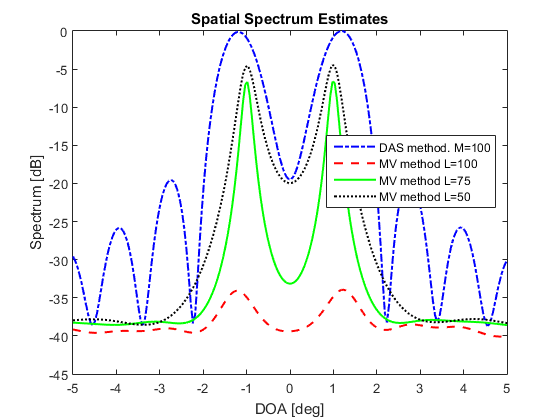
\includegraphics[width=\linewidth]{./images/background/spatial_averaging.png}
    \caption{Effects of spatial smoothing with coherent signals.}
    \label{fig:spatial_smoothing}
\end{figure}


\subsection{Time averaging}
\label{sec:time_averaging}
The MV beamformer has shown to be able to achieve higher resolvability of scatterer points than the conventional DAS. However, the spatial covariance matrix estimate used in the MV beamformer affects the patterns of homogeneous tissue. Homogeneous tissues are typically represented in beamformed images by \textit{speckle}, which consists of the transmitted signals scattered by a large number of small, densely distributed, scatterer points. In this thesis, speckle is generated by simulating a large number of small scatterer points uniformly distributed in the medium.
\cite{speckle} showed that the MV beamformer has a tendency to attenuate the homogeneity of the speckle and may give the impression of scatterer points existing in the homogeneous tissue.
Spatial averaging can enhance scatterer points resolution, but tend to result in lower average speckle magnitude. This effect can be beneficial for certain applications, as it tends to improve the SNR of isolated scatterer points, but can be undesirable in applications that use speckle in their image formation and/or analysis (e.g. skin tissue imaging).

Temporal averaging is a solution proposed by \cite{speckle} to reduce the effect of spatial averaging on speckle. Temporal averaging consists of using multiple samples per range for the spatial covariance matrix estimation. The idea is to allow a better capture of the speckle statistics by using multiple temporal samples, to the expense of reduced spatial resolution in the range dimension. Equation (\ref{eq:mv_temp}) reflects the addition of temporal averaging on Equation (\ref{eq:cov_matrix}):
\begin{equation}
    \boldsymbol{\hat{R}}_{\theta, n} = \frac{1}{(2T + 1) K} \sum_{t=-T}^{T} \sum_{k=0}^{K-1} \boldsymbol{Y_k}[n - t] \boldsymbol{Y_k}^H[n - t],
\label{eq:mv_temp}
\end{equation}
\noindent
where 2T + 1 temporal samples t are used per range unit n.


\subsection{Forward-backward averaging}
\label{sec:fb_averaging}
In Equation (\ref{eq:mv_temp}), each vector $\boldsymbol{Y}_k$ is the vector of time-delayed signals for each array $k$. Those vectors are typically defined as:
\begin{equation}
    \boldsymbol{Y}_k[n] = [y_k[n], y_{k+1}[n],...,y_{k+L-1}[n]], \quad k = 0,...,K-1.
\label{eq:forward_only}
\end{equation}
\noindent
This approach is often referred to as \textit{forward-only} estimate.
On the other hand, any other definition of $\boldsymbol{Y_k}[n]$ can result in a different covariance matrix estimation. Equation (\ref{eq:backward_only}) reflects the definition opted by the \textit{backward-only} approach:
\begin{equation}
    \boldsymbol{Y}_k[n] = [y_{K-k+L-1}[n], y_{K-k+L-2}[n],...,y_{K-k}[n]], \quad k = 0,...,K-1.
\label{eq:backward_only}
\end{equation}
\noindent

The \textit{forward-backward} (FB) averaging is an approach that builds covariance matrix estimates by combining the forward-only and backward-only approaches (\cite{van_trees}):
\begin{equation}
    \boldsymbol{\hat{R}}_{\theta,n}^{FB} = \frac{1}{2} (\boldsymbol{\hat{R}}_{\theta,n}^F + \boldsymbol{\hat{R}}_{\theta,n}^B).
\label{eq:fb_averaging}
\end{equation}

The idea behind the FB approach is to enforce the persymmetric property of the covariance matrix $\boldsymbol{R}$ (Equation (\ref{eq:persymmetric})) and thus removing coherency between the recorded signals.


\subsection{Beamspace projection}
\label{sec:beamspace_projection}
When only imaging a subsection of the whole -90 to 90$^\circ$ angular range, adaptive beamformers can potentially be disturbed by the lack of energy sent and received outside of the image sector.
Diagonal loading (Section \ref{sec:diagonal_loading}) is often applied to ensure some energy distribution along the whole -90 to 90$^\circ$ angular span and render the beamformer's covariance matrix estimate $\boldsymbol{\hat{R}}$ (pseudo-)invertible. Although this approach works, it can be viewed as inefficient, since it can potentially model a much wider image sector than the one actually imaged.

Another approach to making $\boldsymbol{\hat{R}}$ invertible is to reduce the dimensionality of the beamspace model to the one of the imaged sector.
It is worth noting that this approach corrects for the lack of energy outside of the image sector, but does not correct for any potential lack of energy within it. For that reason, diagonal loading is often still used along with beamspace projection.

Transmitted beams are typically both directional and narrow enough so that only a subsection of the image sector is insonated by a single beam. These properties result in most of the energy transmitted by a single beam to be restrained to a relatively small spatial frequency range. With the use of time-delay on received beams, most of this energy can be shifted towards the array's center line, which effectively transposes those spatial frequency ranges to low spatial frequencies. Since then most of the energy lies within low spatial frequencies, one could potentially apply a spatial low-pass filter without losing a lot of information.

This is what beamspace projection conceptually does. The time-delayed signals $\boldsymbol{Y_e}[n]$ can be transposed to a reduced-dimensional beamspace with a simple multiplication by a transformation matrix $\boldsymbol{B}_{bs}$ mapping $\mathbb{C}^M$ to $\mathbb{C}^B$, where $M$ is the number of transducers in the array and $b$ the targeted beamspace dimensionality:
\begin{equation}
    \boldsymbol{Y_e}^b =  \boldsymbol{B}_{bs} \boldsymbol{Y_e}.
\end{equation}
\noindent
The transform can alternatively be applied to the covariance matrix estimate instead of the time-delayed signals:
\begin{equation}
    \boldsymbol{\hat{R}}_{\theta,n}^B =  \boldsymbol{B}_{bs}^T \boldsymbol{\hat{R}}_{\theta,n} \boldsymbol{B}_{bs}.
\end{equation}
\noindent
This is the approach selected in this thesis.
The transformation matrix $\boldsymbol{B}_{bs}$ can be built in several ways. In this thesis, $\boldsymbol{B}_{bs}$ is conceptually built as a spatial lowpass filter, where only the spatial frequencies covering the imaged sector are kept. This approach uses the monochromatic signals assumption presented in Section \ref{sec:beamforming_frequency} which allows to map a physical angle of arrival $\theta$ to a spatial frequency $f_\theta = \sin(\theta) \cdot M / 2$. The reduced-dimensional beamspace should therefore ideally include all spatial frequencies from $0$ to $f_{\theta_{max}}$, where $\theta = 0$ is the direction of the transducers array's normal vector and $\theta_{max}$ is the angle of the imaged sector extremities, and excludes all spatial frequencies $f > f_{\theta_{max}}$.

The number of dimensions $B$ in the projected beamspace should then ideally reflect this condition. If the imaged sector spans the whole $\pm 90^{\circ}$, then the transformation matrix should be the identity matrix, mapping $\mathbb{C}^M$ to $\mathbb{C}^M$, meaning that $B = M$. On the other extreme case, if the image sector consists only of one direction, $\theta = 0$, the resulting beamspace should only have one dimension ($B = 1$). The beamspace dimensionality $B$ can be defined a linear function of $f_{\theta_{max}}$:
\begin{equation}
    B = 2 \cdot f_{\theta_{max}} + 1 = 2 \cdot \frac{\sin(\theta_{max}) \cdot M}{2} + 1,
\label{eq:beamspace_ideal}
\end{equation}
\noindent
where the added 1 represents the central angle $\theta = 0$ and the factor 2 represents the two halves of the image sector. However, the number of dimensions $B$ has to be an integer and $f_{\theta_{max}}$ is not always one. Different rounding approaches can be implemented. In this thesis, the nearest integer higher than $f_{\theta_{max}}$, using the ceiling function, is used to define $B$. The reduced-dimension beamspace then spans a sector bigger or equal to the imaged sector. Equation (\ref{eq:beamspace_ideal}) is redefined accordingly:
\begin{equation}
    B = 2 \cdot \lceil f_{\theta_{max}} \rceil + 1 = 2 \cdot \lceil \frac{\sin(\theta_{max}) \cdot M}{2} \rceil + 1,
\label{eq:beamspace_size}
\end{equation}
\noindent
where $\lceil \rceil$ is the ceiling function.
The transformation matrix $\boldsymbol{B}_{bs}$ is built as a $M x B$ matrix whose columns $b = \{1, 2,..., B \}$ are built as:
\begin{equation}
    \boldsymbol{B}_{bs}(1:M, b) = e^{i \cdot \boldsymbol{n} \cdot \frac{2\cdot \pi}{M} c\cdot (\lfloor B / 2 \rfloor - b)},
\label{eq:beamspace}
\end{equation}
\noindent
where $\boldsymbol{n}$ is a vector of size $M$ containing all integers within the range $[- (L - 1 / 2), L - 1 / 2]$.
In addition to the monochromatic wave assumption, this implementation of $\boldsymbol{B}$ implicitly assumes the beamforming to be working in the far-field (Section \ref{sec:nearfield_farfield}), since it assumes all transducers to experience the same spatial frequency $f_\theta$ for a signal coming from angle $\theta$. 


\subsection{Multibeam covariance matrix approach}
\label{sec:multibeam}
One major drawback to adaptive beamforming methods, in comparison to conventional ones, is their computational complexity. Standard adaptive beamformers compute (and inverse) a separate covariance matrix estimate $\boldsymbol{\hat{R}}_{\theta, n}$ for each image sample, e.i. each radial distance of each received beam. $\boldsymbol{\hat{R}}_{\theta, n}$ is sometimes referred to as \textit{sample covariance matrix}. Since such a matrix is built from a single beam, it also requires the use of spatial averaging (Section \ref{sec:spatial_smoothing}) to decorrelate coherent signals.
\par
Another approach would be to compute a single covariance matrix estimate $\boldsymbol{\hat{R}}_n$ for each radial distance $n$, thus reducing the number of matrix inversions to the number of radial distances (\cite{Jensen_multibeam}). Such a matrix should be formed such that the beamformers weights can be extracted from it for any steering angle $\theta$. This condition is expressed in Equation (\ref{eq:mv_multibeam}), which is Equation (\ref{eq:mv_problem_fixed}) adapted to this situation:
\begin{equation}
    \min_{\boldsymbol{w}} \boldsymbol{w}^H \boldsymbol{\hat{R}}_n \boldsymbol{w}, \quad subject ~ to \quad \boldsymbol{w}^H \boldsymbol{a}_{\theta,n} = 1.
\label{eq:mv_multibeam}
\end{equation}
\noindent
And its solution:
\begin{equation}
    \boldsymbol{w_a} = \frac{\boldsymbol{\hat{R}}_{n}^{-1} \boldsymbol{a_{\theta,n}}}{\boldsymbol{a_{\theta,n}}^H \boldsymbol{\hat{R}}_{n}^{-1} \boldsymbol{a_{\theta,n}}}.
\label{eq:mvmb_weight}
\end{equation}
\noindent
It is worth mentioning that phase-based focusing is working under the assumption of narrowband signals. Although this assumption usually does not hold in medical ultrasound imaging, phase-based focusing can be done for small phase shifts. This issue is explained in more details in Section \ref{sec:beamforming_frequency}.

Let the set of time- and phase-delayed signals $\boldsymbol{\hat{Y}}_n$ be defined as:
\begin{equation}
    \boldsymbol{\hat{Y}}_n = \boldsymbol{A}_n \circ \boldsymbol{Y}_n, 
\label{eq:time_phase_delayed}
\end{equation}
\noindent
where $\boldsymbol{A_n}$ is a the set of steering vectors $\boldsymbol{a_{\theta, n}}$ for any given radius index $n$ and $\circ$ denotes the Hadamard product.
The covariance matrix estimate $\boldsymbol{\hat{R}_n}$ can then be formed from $\boldsymbol{\hat{Y}}_n$:
\begin{equation}
    \boldsymbol{\hat{R}}_n = \frac{1}{S} \boldsymbol{\hat{Y}}_n^T \boldsymbol{\hat{Y}}_n,
\label{eq:mb_covariance}
\end{equation}
\noindent
where $S$ is the number of received beams steering angles $(\theta_1,..., \theta_S)$.
This \textit{approach to multibeam covariance matrices} is often simply referred to as the \textit{multibeam} approach, and beamformers using this approach as \textit{multibeam beamformers}.

Once the adaptive array weights are extracted from the covariance matrix estimate, they can actually be used in multiple ways. The most straightforward use is the \textit{single-beam (SB) output}. An image sample $Z_{\theta,n}$ is created by applying the weights $\boldsymbol{w}_{\boldsymbol{a}}$, coming from Equation (\ref{eq:mvmb_weight}) with steering vector $\boldsymbol{a_{\theta,n}}$, to its corresponding array sample $\bar{Y}_{\boldsymbol{a}}$:
\begin{equation}
    Z_{\theta,n} = | \boldsymbol{w_a}^T \boldsymbol{\hat{Y}}_{\theta, n} |^2.
\end{equation}
\noindent
However, due to the adaptive nature of the beamformer, the recorded data used for different directions than that of the image sample can also hold information for that direction.
An alternative approach known as \textit{multibeam compound (MBC) output}, or \textit{multibeam (MB) output} forms an image sample based on the whole covariance matrix estimate rather than a single array sample:
\begin{equation}
    Z_{\theta,n} = \boldsymbol{w_a}^T \boldsymbol{\hat{R}}_n \boldsymbol{w_a}.
\end{equation}


\subsection{Iterative Adaptive Approach (IAA)}
\label{sec:IAA}
As stated in the introduction of this thesis, adaptive beamformers are still nowadays struggling to truly emerge as commercial products in medical ultrasound imaging. This has arguably been mainly due to their global reduced robustness compared to those of the conventional beamformers, their increased computational load, making real-time imaging difficult, and the introduction of additional user parameters to control their degree of adaptivity, which makes them much more difficult to use without a profound knowledge of how they work. 

As the available computational capacities are constantly improving, the computational load issue is becoming less of a concern. It has actually recently been shown that adaptive beamforming (MV) can now be used for real-time imaging when implemented in a Graphics Processing Unit (GPU) framework (\cite{GPU}).
The introduction of various robustification methods allows for more stable beamformers, often at the cost of reduced resolution capacity and increased computational load. However, those methods have to be precisely calibrated in order to yield optimum results. This typically restrains the use of such beamformers to people trained in the domain of beamforming.

In order to limit this parametrization burden, new approaches to adaptive beamforming have emerged and are often referred to as \textit{parameter-free} approaches (\cite{Yardibi_nonparametric_IAA, Yardibi, Du_parameter_free, Jensen_IAA}). This thesis builds on the \textit{Iterative Adaptive Approach} (IAA) as presented by \cite{Jensen_IAA}. IAA is based on the \textit{sparse signal representation} (\cite{Yardibi_nonparametric_IAA}), as it models a number of potential reflector in the imaged medium often much denser than the actual number of sources. The received signal of any potential source $q$ can be modeled as:
\begin{equation}
    \boldsymbol{y}_q(t) = s_q(t)  \boldsymbol{a}_q,
\end{equation}
\noindent
where $s_q(t)$ is the source's signal and $\boldsymbol{a}_q$ is the phase-based steering vector pointing to the location of the source $q$. The covariance matrix of a single source is then:
\begin{equation}
    \boldsymbol{R}_q = \boldsymbol{E}[\boldsymbol{y}_q(t) \boldsymbol{y}_q(t)^T] = |s_q(t)|^2 \boldsymbol{a}_q \boldsymbol{a}_q^T.
\end{equation}

\noindent
The IAA beamformers follows the sparse signal representation and models $Q$ sources spread densely across the image sector. Assuming those sources are uncorrelated, the total covariance matrix $\boldsymbol{R}$ is the sum of $\boldsymbol{R}_q$ for each source $q$:
\begin{equation}
    \boldsymbol{R} = \sum_{q=1}^{Q} |s_q|^2 \boldsymbol{a}_q \boldsymbol{a}_q^T = \boldsymbol{A} \boldsymbol{P} \boldsymbol{A}^T,
\label{eq:R_IAA}
\end{equation}
\noindent
where $\boldsymbol{A}$ is the matrix of steering vectors $\boldsymbol{a}_q$ and $\boldsymbol{P}$ is a $Q x Q$ diagonal matrix with the sources' squared amplitudes $|s_q|^2$ along its diagonal.
The IAA output image $\boldsymbol{Z}$ is formed from the estimated sources amplitudes $|s_q|$. Therefore each image sample $\boldsymbol{Z}_{\theta,n}$ is build from the corresponding $\boldsymbol{P}$ diagonal element $\boldsymbol{P}_{qq}$ for $q$ being the source located at $(\theta,n)$:
\begin{equation}
    Z_{\theta,n} = \sqrt{\boldsymbol{P}_{qq}}.
\label{eq:IAA_output}
\end{equation}
\noindent
Given an estimate $\boldsymbol{\hat{R}}$ of the covariance matrix $\boldsymbol{R}$, an initial estimate of $\boldsymbol{P}$ can be built by applying matched spatial filtering:
\begin{equation}
    \boldsymbol{\hat{P}} = \boldsymbol{A}_n^T \boldsymbol{\hat{R}} \boldsymbol{A}_n.
\end{equation}

\noindent
This initial estimate of $\boldsymbol{P}$ actually corresponds to the output of the DAS beamformer (Equation (\ref{eq:das_power})) using the multibeam covariance matrix estimation approach (Section \ref{sec:multibeam}).
The iterative stage improves this estimate of $\boldsymbol{P}$ by iteratively using the MV beamformer (Section \ref{sec:MV}):
\begin{enumerate}
    \item The covariance matrix model $\boldsymbol{\bar{R}}$ is built from Equation (\ref{eq:R_IAA}) using $\boldsymbol{\hat{P}}$.
    \item For each potential source $q$, a new set of weights $\boldsymbol{w}_q$ is built using the MV beamformer (Equation (\ref{eq:mv_weight})).
    \item Those weights $\boldsymbol{w}_q$ are then used to form new estimates of the sources' squared amplitudes:
    \begin{equation}
        \boldsymbol{\hat{P}}_{qq} = \boldsymbol{w}_q^T \boldsymbol{\hat{R}} \boldsymbol{w}_q.
    \label{eq:mb_output}
    \end{equation}
\end{enumerate}

The last step of the iteration is obviously also based on the multibeam approach, but $\boldsymbol{\hat{P}}_{qq}$ can also be estimated based on the singlebeam approach:
\begin{equation}
    \boldsymbol{\hat{P}}_{qq} = |\boldsymbol{w}_q^T \boldsymbol{\hat{Y}}_q |^2,
\label{eq:sb_output}
\end{equation}
\noindent
where $\boldsymbol{\hat{Y}}_q$ is the set of data recorded by the array's transducers and time- and/or phase-shifted in order to align the focus of the array to the position of source $q$. This approach is referred to as the single-beam (SB) output, whereas Equation (\ref{eq:mb_output}) is referred to as the multibeam compound (MBC) or multibeam (MB) output (\cite{Jensen_multibeam, Jensen_IAA}).

After some iterations, the algorithm converges and $\boldsymbol{\hat{P}}$ can used in Equation (\ref{eq:IAA_output}) to build a beamformed image.
The iteration stop condition can either be a fixed number of iterations, a convergence threshold or a combination of both.
The studies by \cite{Yardibi_nonparametric_IAA} and \cite{Jensen_IAA} empirically show reasonable convergences after 5 to 15 iterations (SB: 10-15, MB: 5-10).

Although the choice of SB or MB output approach can be preserved for the last estimate of $\boldsymbol{P}$, it does not have to be either. Regardless of which approach is applied during the iteration stage, the same dilemma occurs when building the beamformed image samples. This combination of choices results in four possible variants of the IAA algorithm:
\begin{itemize}
    \item IAA-SB/SB: The SB approach is used both during the iteration stage and the final sources amplitude estimation.
    \item IAA-SB/MB: The SB approach is used during the iteration stage and the MB approach for the final sources amplitude estimation.
    \item IAA-MB/SB: The MB approach is used during the iteration stage and the SB approach for the final sources amplitude estimation.
    \item IAA-MB/MB: The MB approach is used both during the iteration stage and the final sources amplitude estimation.
\end{itemize}
\noindent
In this thesis, we focus on the multibeam output approach during the iteration process, so we only implement the last two variants of the IAA algorithm.
To avoid confusing, we refer to them as IAA-MBSB, respectively IAA-MBMB, and simply IAA-MB when referring to both approaches.
